\documentclass[pdf,azure,slideColor,colorBG]{prosper}

\usepackage[latin1]{inputenc}
\usepackage{pstricks,pst-node,pst-text,pst-3d}
\usepackage{amsmath}
\usepackage{graphics}
\usepackage{multicol}

\makeatletter
\define@key{PDF}{Movie}{\pdf@addtoks{#1}{Movie}}
\define@key{PDF}{Activation}{\pdf@addtoks{#1}{Activation}}
\newcommand{\moviewithpreview}[3]{% args: width, preview, movie
    \pdfmark[{\includegraphics[width=#1]{#2}}]{%
    pdfmark=/ANN,Subtype=/Movie,Movie=<< /F (#3) >>,%
    Activation=<< /ShowControls true /Mode /Repeat >>}}
\newcommand{\movie}[3]{% args:width, height, movie
    \pdfmark[{\hbox to #1 {\vbox to #2 { }}}]{%
    pdfmark=/ANN,Subtype=/Movie,Movie=<< /F (#3) /Poster true >>,%
    Activation=<< /ShowControls true /Mode /Repeat >>}}

% Args: width, preview, movie
\newcommand{\hrefWithPreview}[3]{%
  \href{#3}{\includegraphics[width=#1]{#2}}
}
%
\makeatother


\Logo{
\includegraphics[width=3cm]{nrc_newlogo.ps}}

\title{Simulating Focal Plane Array Observations with MeqTrees}
\author{\green Tony Willis} 
\email{tony.willis@nrc.ca}
\institution{ 
  National Research Council of Canada \\ Herzberg Institute of Astrophysics \\
  Penticton, BC, Canada V2A 6J9
}

\ptsize{10}
\begin{document}
\maketitle


%%%%%%%%%%%%%%%%%%%%%%%%%%%%%%%%%%%%%%%%%%%%%%%%%%%%%%%%%%%%%%%%%%%%%%%%%
%%% TeX definitions of mathematical symbols and names used for the %%%%%% 
%%% Measuerement Equation of Generic Interferometer (MEGI)  %%%%%%%%%%%%%
%%%%%%%%%%%%%%%%%%%%%%%%%%%%%%%%%%%%%%%%%%%%%%%%%%%%%%%%%%%%%%%%%%%%%%%%%
\def\thisfile{~/aips++/nfra/megi-symbols.tex}

% The following list is available as a LaTeX list of definitions. It
% could be the start of an official AIPS++ list of symbol names, to
% encourage (enforce?) consistency in all AIPS++ documents and code.

%%%%%%%%%%%%%%%%%%%%%%%%%%%%%%%%%%%%%%%%%%%%%%%%%%%%%%%%%%%%%%%%%%%%%%%%%
%   Some user-defined TeX commands:

\newcommand{\tbt}[4]
  {\left(\begin{array}{cc}#1 & #2\\ #3 & #4 \end{array}\right)}
\newcommand{\ddp}[2]{\frac {\partial #1}{\partial #2}}
\newcommand{\ddpn}[3]{\frac {\partial^{#3}{#1}}{\partial{#2}^{#3}}}
\newcommand{\dirprod}[2]{{#1}\otimes{#2}^\ast}


%%%%%%%%%%%%%%%%%%%%%%%%%%%%%%%%%%%%%%%%%%%%%%%%%%%%%%%%%%%%%%%%%%%%%%%%%
%   Naming system (method in the madness):

% \mmName              % Matrix 
% \mjName              % Jones matrix (2x2)
% \vvName              % Vector 

% \ssName              % subscript or superscript (e.g. \ssI: \Feed I)
% \ccName              % Coordinate (e.g. \ccL: Sky L-coordinate)
% \aaName              % Projected angle (e.g. \aaXY: from X-axis to Y-axis)

% \ppName              % Parameter  

% I,J                  % \Feed labels (e.g. \FeedI)
% X,Y,R,L              % Polarisation labels
% A,B                  % \Receptor labels (e.g. \RcpB)
% P,Q                  % \IFout labels (e.g. \IFP)
%%%%%%%%%%%%%%%%%%%%%%%%%%%%%%%%%%%%%%%%%%%%%%%%%%%%%%%%%%%%%%%%%%%%%%%%%

%  \gloshead{Names of things for which there is a precise definition}
%   NB: Use a closing backslash (e.g. `\Receptot\ ') for interword space! 
  
\def\Receptor{{\sl receptor}}     % Converts field to voltage (e.g. dipole) 
\def\Receptors{{{\Receptor}s}}    %   plural   

\def\Feed{{\sl feed}}             % Logical e.m.-to-signal converter 
\def\Feeds{{{\Feed}s}}            %   plural  

\def\Station{{\sl station}}       % Logical component of a synthesis telescope
\def\Stations{{{\Station}s}}      %   plural  

\def\Antenna{{\sl antenna}}       % Physical grouping of Feeds
\def\Antennas{{{\Antenna}s}}      %   plural  

\def\IFchannel{{\sl IF-channel}}  % Signal outputs from an \Feed 
\def\IFchannels{{{\IFchannel}s}}  %   plural 
\def\IFout{{\IFchannel}}          % Old symbol (still supported) 
\def\IFouts{{\IFchannels}}        %   plural 

\def\Telescope{{\sl telescope}}   % Entire instrument (e.g. WSRT, GBT)
\def\Telescopes{{\Telescope}s}    %   plural 

\def\Interferometer{{\sl interferometer}}  % Two \IFout's or two \Feed's
\def\Interferometers{{{\Interferometer}s}} %   plural

\def\Visibility{{\sl visibility}}     % 1-4 complex spectra, 
\def\Visibilities{{\sl visibilities}} %   plural 
                                  % output of an \Interferometer. 
\def\Projected{{\sl projected}}   % Projected on sky plane (or on the
                                  % plane perpendicular to propagation)


%  \gloshead{Labels:}

\def\FeedI{{\sf i}}       % The `first' \Feed in an interferometer
\def\FeedJ{{\sf j}}       % The `second' \Feed in an interferometer
\def\StationI{{\sf i}}    % The `first' \Station in an interferometer
\def\StationJ{{\sf j}}    % The `second' \Station in an interferometer
\def\AntI{{\FeedI}}        %   old symbol, still supported
\def\AntJ{{\FeedJ}}        %   old symbol, still supported

\def\RcpA{{\sf a}}        % The `first' dipole in a \Feed
\def\RcpB{{\sf b}}        % The `second' dipole in a \Feed

\def\IFP{{\sf p}}         % The `first' IF-channel from a \Feed
\def\IFQ{{\sf q}}         % The `second' IF-channel from a \Feed

\def\RPol{{\sf r}}        % r-pol 
\def\LPol{{\sf l}}        % l-pol 

\def\XPol{{\ccX}}         % x-pol 
\def\YPol{{\ccY}}         % y-pol 

%  \gloshead{Coordinate frames:}

\def\ccT{{\sf t}}                   % time-coord 
\def\ccF{{\sf f}}                   % frequency-coord 

%  Polarisation-frame (for electric polarisation vector):

\def\ccX{{\sf x}}                   % x-coord 
\def\ccY{{\sf y}}                   % y-coord
\def\ccZ{{\sf z}}                   % y-coord

\def\ccXPol{{\XPol}}                % x-pol-coord 
\def\ccYPol{{\YPol}}                % y-pol-coord
\def\ccRPol{{\RPol}}                % r-pol-coord 
\def\ccLPol{{\LPol}}                % l-pol-coord

%  Array-frame (for baseline vector):

\def\ccU{{\sf u}}                   % u-coord 
\def\ccV{{\sf v}}                   % v-coord 
\def\ccW{{\sf w}}                   % w-coord  
\def\vvUVW{{\vec{u}}}               % Projected baseline vector

\def\ccGX{{\sf x}}                  % antenna position coord 
\def\ccGY{{\sf y}}                  % antenna position coord 
\def\ccGZ{{\sf z}}                  % antenna position coord 

\def\vvAntPos{{\vec{r}}}       % Projected `Antenna' position vector 
                               %   (Receptor phase centre?)
\def\vvAntPosEl{{\sf r}}       %   element

%  Sky coord. frame (source positions) w.r.t. Delay Centre:  

\def\ccL{{\sf l}}                   % l-coord 
\def\ccM{{\sf m}}                   % m-coord 
\def\ccN{{\sf n}}                   % n-coord (=sqrt[1-l^2-m^2]) 

\def\vvLMN{{\vec{\rho}}}            % Vector (l,m) in Sky frame 
\def\vvFTC{{\vvLMN_{ftc}}}          % Fringe Tracking Centre (l,m,f) 
\def\vvMC{{\vvLMN_{mc}}}            % Map centre (l,m) 

%  Antenna coord. frame (l',m'), projected on the Sky:

\def\ccLI{{\ccL^{'}_{\FeedI}}}       % l'-coord of \Feed-frame  
\def\ccMI{{\ccM^{'}_{\FeedI}}}       % m'-coord 
\def\ccLIO{{\ccL_{\FeedI{0}}}}       % l-coord of origin of \Feed-frame i
\def\ccMIO{{\ccM_{\FeedI{0}}}}       % m-coord 

%  Receptor coord. frames (l'',m''), projected on the Sky:

\def\ccLIA{{\ccL^{''}_{{\FeedI\RcpA}}}}  % l''-coord for \RcpA-frame 
\def\ccMIA{{\ccM^{''}_{{\FeedI\RcpA}}}}  % m''-coord 
\def\ccLIAO{{\ccLI_{\RcpA{0}}}}         % l'-coord of origin of \RcpA-frame 
\def\ccMIAO{{\ccMI_{\RcpA{0}}}}         % m'-coord 

\def\ccLIB{{\ccL^{''}_{{\FeedI\RcpB}}}}  % l''-coord for \RcpB-frame 
\def\ccMIB{{\ccM^{''}_{{\FeedI\RcpB}}}}  % m''-coord 
\def\ccLIBO{{\ccLI_{\RcpB{0}}}}         % l'-coord of origin of \RcpB-frame 
\def\ccMIBO{{\ccMI_{\RcpB{0}}}}         % m'-coord 

%  Projected angles between the various coord frames: 

\def\aaProj{{\gamma}}                % Projected angle 

\def\aaXY{{\aaProj_{\ccX\ccY}}}      % from Pol x-axis to Pol y-axis 
\def\aaLM{{\aaProj_{\ccL\ccM}}}      % from Sky l-axis to Sky m-axis 
\def\aaLX{{\aaProj_{\ccL\ccX}}}      % from Sky l-axis to Pol x-axis 
\def\aaLI{{\aaProj_{\ccL\FeedI}}}     % from Sky l-axis to \Feed l'-axis 
\def\aaIA{{\aaProj_{\FeedI\RcpA}}}    % from \Feed l'-axis to \RcpA l''-axis 
\def\aaIB{{\aaProj_{\FeedI\RcpB}}}    % from \Feed l'-axis to \RcpB l''-axis 

\def\aaXI{{\aaProj_{\ccX\FeedI}}}     % from x-axis to \Feed l'-axis 
\def\aaXA{{\aaProj_{\ccX\RcpA}}}     % from x-axis to \RcpA l''-axis 
\def\aaYB{{\aaProj_{\ccY\RcpB}}}     % from y-axis (!) to \RcpB l''-axis  

\def\aaXYexp{{\pi/2}}                % from x-axis to y-axis 
\def\aaLMexp{{\pi/2}}                % from l-axis to m-axis
\def\aaLXexp{{\pi/2}}                % from l-axis to x-axis 
\def\aaXIexp{{-\aaLX+\aaLI}}                % x to l' 
\def\aaXAexp{{-\aaLX+\aaLI+\aaIA}}          % x to l''(A)  
\def\aaYBexp{{-\aaXY-\aaLX+\aaLI+\aaIB}}    % x to l''(B) 


%  \gloshead{Miscellaneous parameters:}

\def\ppHA{{HA}}                  % Hour Angle
\def\ppDEC{{DEC}}                % Declination
\def\ppRA{{RA}}                  % Right Ascension
\def\ppLAT{{LAT}}                % Latitude (on the Earth)
\def\ppParall{{\beta}}           % parallactic angle (between great
			         % circles through North Pole and Zenith)

\def\ppFarad{{\chi}}             % Faraday rotation angle (rad)
\def\ppAmpl{{a}}                 % Amplitude
\def\ppPhase{{\psi}}             % Phase
\def\ppPhaseZero{{\zeta}}        % Phase-zero
\def\ppRcpPosDev{{\phi}}	 % \Receptor pos. angle deviation  
\def\ppRcpEllDev{{\theta}}       % \Receptor ellipticity deviation
\def\ppDiposErr{{\ppRcpPosDev}}	 %  old symbol, still supported  
\def\ppEllipt{{\ppRcpEllDev}}    %  old symbol, still supported

\def\ppBellipt{{\epsilon}}       % beam ellipticity (shape) factor      
\def\ppBsigma{{\sigma}}          % sigma of gaussian beam       

%  \gloshead{Jones Matrices (2x2):}

\def\mjJones{{\sf J}}          % Jones instrumental response matrix
\def\mjJonesEl{{\sf j}}        %   matrix element

\def\mjFrot{{\sf F}}           % Faraday rotation matrix
\def\mjFrotEl{{\sf f}}         %   matrix element of \mjFrot

\def\mjTrop{{\sf T}}           % Atmospheric gain matrix
\def\mjTropEl{{\sf t}}         %   matrix element of \mjGatm
\def\mjGatm{{\mjTrop}}         % Old symbol, still supported
\def\mjGatmEl{{\mjTropEl}}     % Old symbol, still supported

\def\mjKern{{\sf K}}           % Fourier Transform kernel matrix  
\def\mjKernEl{{\sf k}}         %   matrix element
\def\mjKref{{\mjKern^0}}       % FT kernel for field centre  
\def\mjKrefEl{{\mjKernEl^0}}   %   matrix element  
\def\mjKoff{{\mjKern^{'}}}     % For source, relative to field centre  
\def\mjKoffEl{{\mjKernEl^{'}}} %   matrix element  
\def\mjWarr{{\mjKern}}         % Old symbol (used to be \sf W)  
\def\mjWarrEl{{\mjKernEl}}     % Old symbol (used to be \sf w)  

\def\mjProj{{\sf P}}           % Receptor projection angle w.r.t. Sky 
\def\mjProjEl{{\sf p}}         %   matrix element 
\def\mjPrcp{{\mjProj}}         % Old symbol, still supported 
\def\mjPrcpEl{{\mjProjEl}}     % Old symbol, still supported  

\def\mjBtot{{\sf B}}           % Total Voltage Pattern (=DPE)
\def\mjBtotEl{{\sf b}}         %   matrix element of \mjBtot
\def\mjBeam{{\sf E}}           % Antenna Voltage Beam matrix 
\def\mjBeamEl{{\sf e}}         %   matrix element of \mjBeam
% \def\mjBatt{{\sf B}}           % Attenuation beam matrix (obsolete)
% \def\mjBattEl{{\sf b}}         %   matrix element of \mjBatt
% \def\mjObst{{\sf O}}           % Beam obstruction effect matrix (obsolete)
% \def\mjObstEl{{\sf o}}         %   matrix element of \mjObst

\def\mjConf{{\sf C}}           % configuration matrix
\def\mjConfEl{{\sf c}}         %   matrix element

\def\mjDrcp{{\sf D}}           % \Receptor cross-`leakage' matrix
\def\mjDrcpEl{{\sf d}}         %   matrix element of \mjDrcp
\def\mjLeak{{\mjDrcp}}         % Old symbol, still supported
\def\mjLeakEl{{\mjDrcpEl}}     % Old symbol, still supported

\def\mjHybr{{\sf H}}           % Hybrid network matrix (linear to circular)
\def\mjHybrEl{{\sf h}}         %   matrix element

\def\mjComm{{\sf Y}}           % signal-channel commutation matrix
\def\mjCommEl{{\sf y}}         %   matrix element

\def\mjZpzd{{\sf Z}}           % Phase Zero Difference matrix
\def\mjZpzdEl{{\sf z}}         %   matrix element

\def\mjGrec{{\sf G}}           % Receiver Gain matrix (electronics)
\def\mjGrecEl{{\sf g}}         %   matrix element

\def\mjQsum{{\sf Q}}           % Receiver gain of sum-output of tied array 
\def\mjQsumEl{{\sf q}}         %   matrix element
\def\mjGsum{{\mjQsum}}         % Old symbol, still supported 
\def\mjGsumEl{{\mjQsumEl}}     % Old symbol, still supported 


%  \gloshead{Other ME matrices and vectors:} 

\def\mmZero{{\sf Zero}}        % Zero matrix 
\def\mmUnit{{\cal U}}          % Unit matrix 
\def\mmDiag{{\sf Diag}}        % Diagonal matrix 
\def\mmMult{{\sf Mult}}        % Multiplication/magnification matrix 
\def\mjZero{{\mmZero}}         % 2x2 Zero matrix 
\def\mjUnit{{\mmUnit}}         % 2x2 Unit matrix 
\def\mjDiag{{\mmDiag}}         % 2x2 Diagonal matrix D(a,b)
\def\mjMult{{\mmMult}}         % 2x2 Multiplication matrix M(a)=D(a,a)=a.U
\def\mjRot{{\sf Rot}}          % 2x2 rotation matrix R(alpha[,beta])
\def\mjEll{{\sf Ell}}          % 2x2 Ellipticity matrix E(alpha[,beta])
\def\mjLtoC{{\cal H}}          % 2x2 Conversion from Linear to Circular pol
\def\mjCtoL{{\mjLtoC^{-1}}}    % 2x2 Conversion from Circular to Linear pol

\def\vvZero{{\vec{0}}}         % Zero vector

\def\vvIQUV{{\vec{I}}}         % Stokes vector (I,Q,U,V)

\def\vvCoh{{\vec{V}}}          % Visibility (`coherency') vector (2-4)
\def\vvCohEl{{\sf v}}          %   element of \vvCoh

\def\vvElec{{\vec{E}}}         % Electric field vector (2-4)
\def\vvElecEl{{\sf e}}         %   element of \vvElec

\def\vvAifr{{\vec{A}}}         % Additive ifr-based vector (4)
\def\vvAifrEl{{\sf a}}         %   element of \vvAifr

\def\mmStokes{{\sf S}}         % Stokes conversion matrix (4x4) to Coherence

\def\mmMueller{{\cal M}}       % Mueller matrix (Stokes to Stokes)

\def\mmXifr{{\sf X}}           % Correlator matrix (ifr-based) 
\def\mmXifrEl{{\sf x}}         %   element of matrix \mmXAifr

\def\mmMifr{{\sf M}}           % Multiplicative ifr-based gain 
\def\mmMifrEl{{\sf m}}         %   element of matrix \mmMAifr




%%%%%%%%%%%%%%%%%%%%%%%%%%%%%%%%%%%%%%%%%%%%%%%%%%%%%%%%%%%%%%%%%%%%%%%%
%%%%%%%%%%%%%%%%%%%%%%%%%%%%%%%%%%%%%%%%%%%%%%%%%%%%%%%%%%%%%%%%%%%%%%%%
%  Secondary symbols (much-used combinations of the basic symbols above)
%%%%%%%%%%%%%%%%%%%%%%%%%%%%%%%%%%%%%%%%%%%%%%%%%%%%%%%%%%%%%%%%%%%%%%%%


\def\ssI{_{\FeedI}}                % subscript \Feed I  
\def\ssJ{_{\FeedJ}}                % subscript \Feed J  
\def\ssIn{_{\FeedI n}}             % subscript  
\def\ssJm{_{\FeedJ m}}             % subscript  
\def\ssIk{_{\FeedI k}}             % subscript  
\def\ssJk{_{\FeedJ k}}             % subscript  
\def\ssInk{_{\FeedI nk}}           % subscript  
\def\ssJmk{_{\FeedJ mk}}           % subscript  

\def\ssP{_{\IFP}}                 % subscript \IFout P  
\def\ssQ{_{\IFQ}}                 % subscript \IFout Q 
\def\ssA{_{\RcpA}}                % subscript \Receptor A 
\def\ssB{_{\RcpB}}                % subscript \Receptor B 

\def\ssX{_{\XPol}}                % subscript   
\def\ssY{_{\YPol}}                % subscript   
\def\ssR{_{\RPol}}                % subscript   
\def\ssL{_{\LPol}}                % subscript   

\def\ssLin{^{+}}                  % superscript for linear pol  
\def\ssLI{^{+}_{\FeedI}}           % sub/super  
\def\ssLJ{^{+}_{\FeedJ}}           % sub/super  
\def\ssLIJ{^{+}_{\FeedI\FeedJ}}     % sub/super  
\def\ssLIA{^{+}_{\FeedI\RcpA}}     % sub/super  
\def\ssLIB{^{+}_{\FeedI\RcpB}}     % sub/super  
\def\ssCir{^{\odot}}              % superscript for circular pol  
\def\ssCI{^{\odot}_{\FeedI}}       % sub/super  
\def\ssCJ{^{\odot}_{\FeedJ}}       % sub/super  
\def\ssCIJ{^{\odot}_{\FeedI\FeedJ}} % sub/super  
\def\ssCIA{^{\odot}_{\FeedI\RcpA}} % sub/super  
\def\ssCIB{^{\odot}_{\FeedI\RcpB}} % sub/super  

\def\ssVI{^{vis}_{\FeedI}}         % sub/super  
\def\ssSI{^{sky}_{\FeedI}}         % sub/super  
\def\ssVIn{^{vis}_{\FeedI n}}      % sub/super  
\def\ssSIn{^{sky}_{\FeedI n}}      % sub/super  
\def\ssSInk{^{sky}_{\FeedI nk}}    % sub/super  
\def\ssVJ{^{vis}_{\FeedJ}}         % sub/super  
\def\ssSJ{^{sky}_{\FeedJ}}         % sub/super  
\def\ssVJm{^{vis}_{\FeedJ m}}      % sub/super  
\def\ssSJm{^{sky}_{\FeedJ m}}      % sub/super  
\def\ssSJmk{^{sky}_{\FeedJ mk}}    % sub/super  

\def\ssIX{_{\FeedI\XPol}}          % subscript   
\def\ssIY{_{\FeedI\YPol}}          % subscript   
\def\ssIR{_{\FeedI\RPol}}          % subscript   
\def\ssIL{_{\FeedI\LPol}}          % subscript   
\def\ssIA{_{\FeedI\RcpA}}          % subscript   
\def\ssIB{_{\FeedI\RcpB}}          % subscript   
\def\ssIP{_{\FeedI\IFP}}           % subscript   
\def\ssIQ{_{\FeedI\IFQ}}           % subscript   

\def\ssIJ{_{\FeedI\FeedJ}}          % subscript 
\def\ssXY{_{\XPol\YPol}}          % subscript   
\def\ssRL{_{\RPol\LPol}}          % subscript   
\def\ssAB{_{\RcpA\RcpB}}          % subscript   
\def\ssPQ{_{\IFP\IFQ}}            % subscript 

\def\ssIXX{_{\FeedI\XPol\XPol}}    % subscript   
\def\ssIYX{_{\FeedI\YPol\XPol}}    % subscript   
\def\ssIXY{_{\FeedI\XPol\YPol}}    % subscript   
\def\ssIYY{_{\FeedI\YPol\YPol}}    % subscript   

\def\ssIRR{_{\FeedI\RPol\RPol}}    % subscript   
\def\ssILR{_{\FeedI\LPol\RPol}}    % subscript   
\def\ssIRL{_{\FeedI\RPol\LPol}}    % subscript   
\def\ssILL{_{\FeedI\LPol\LPol}}    % subscript   

\def\ssIXA{_{\FeedI\XPol\RcpA}}    % subscript   
\def\ssIYA{_{\FeedI\YPol\RcpA}}    % subscript   
\def\ssIXB{_{\FeedI\XPol\RcpB}}    % subscript   
\def\ssIYB{_{\FeedI\YPol\RcpB}}    % subscript   

\def\ssIRA{_{\FeedI\RPol\RcpA}}    % subscript   
\def\ssILA{_{\FeedI\LPol\RcpA}}    % subscript   
\def\ssIRB{_{\FeedI\RPol\RcpB}}    % subscript   
\def\ssILB{_{\FeedI\LPol\RcpB}}    % subscript   

\def\ssIAA{_{\FeedI\RcpA\RcpA}}    % subscript   
\def\ssIBA{_{\FeedI\RcpB\RcpA}}    % subscript   
\def\ssIAB{_{\FeedI\RcpA\RcpB}}    % subscript   
\def\ssIBB{_{\FeedI\RcpB\RcpB}}    % subscript   

\def\ssIAP{_{\FeedI\RcpA\IFP}}     % subscript  
\def\ssIBP{_{\FeedI\RcpB\IFP}}     % subscript  
\def\ssIAQ{_{\FeedI\RcpA\IFQ}}     % subscript  
\def\ssIBQ{_{\FeedI\RcpB\IFQ}}     % subscript  

\def\ssIPP{_{\FeedI\IFP\IFP}}      % subscript 
\def\ssIQP{_{\FeedI\IFQ\IFP}}      % subscript 
\def\ssIPQ{_{\FeedI\IFP\IFQ}}      % subscript 
\def\ssIQQ{_{\FeedI\IFQ\IFQ}}      % subscript 
   
\def\ssIPJP{_{\FeedI\IFP\,\FeedJ\IFP}}     % subscript 
\def\ssIPJQ{_{\FeedI\IFP\,\FeedJ\IFQ}}     % subscript 
\def\ssIQJP{_{\FeedI\IFQ\,\FeedJ\IFP}}     % subscript 
\def\ssIQJQ{_{\FeedI\IFQ\,\FeedJ\IFQ}}     % subscript 


%%%%%%%%%%%%%%%%%%%%%%%%%%%%%%%%%%%%%%%%%%%%%%%%%%%%%%%%%%%%%%%%%%%%%%%%%
%%% End of MEGI symbols definition file megi-symbols.tex %%%%%%%%%%%%%%%%
%%%%%%%%%%%%%%%%%%%%%%%%%%%%%%%%%%%%%%%%%%%%%%%%%%%%%%%%%%%%%%%%%%%%%%%%%
































































%---------------------------------------------------------------------- SLIDE -
\begin{slide}{Topics}
\begin{small}
\begin{itemize}
\item Overview of Measurement Equation
\item Overview of MeqTrees
\item Example of MeqTrees Configuration
\item Correction for E-Jones effects
\item Simulation Setup
\item Examples of MeqTrees Simulations
\begin{itemize}
\item Phase-Conjugate Weighting
\item Optimization for Gaussian beam shape
\item AzEl observation tracking a fixed offset position
\end{itemize}
\item What's Next?
\end{itemize}
\end{small}
\end{slide}
%------------------------------------------------------------------------------

%---------------------------------------------------------------------- SLIDE -
\begin{slide}{Measurement Equation - HBS}
{\centering
\resizebox*{0.6\columnwidth}{!}{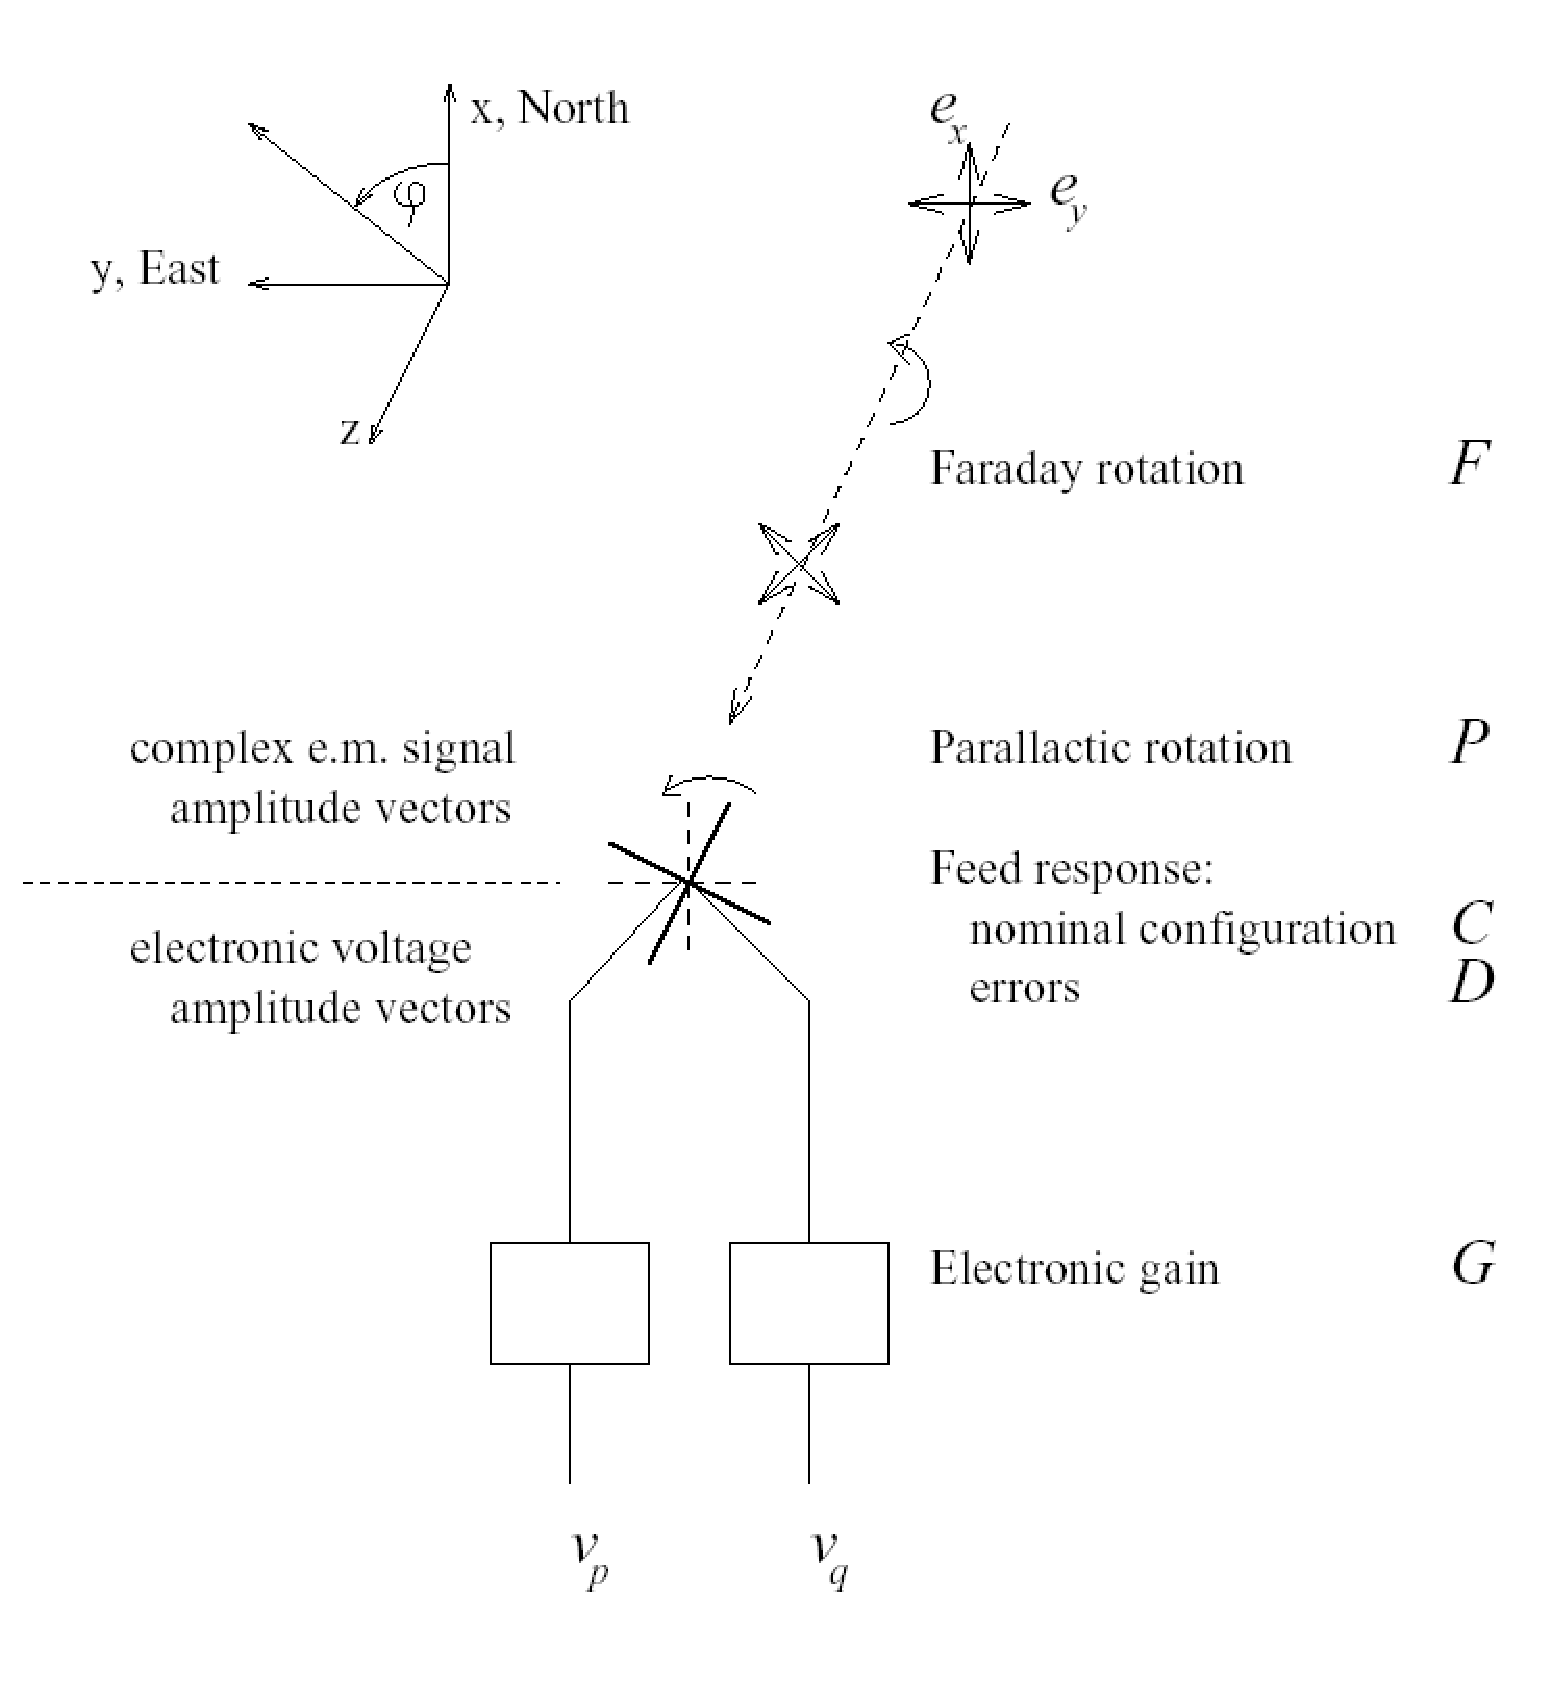
\includegraphics{schematic_transformations.ps}}
\par}
\end{slide}
%------------------------------------------------------------------------------

%---------------------------------------------------------------------- SLIDE -

\begin{slide}{Jones Matrices}
\begin{small}
\begin{itemize}
\item The real heart of the Measurement Equation (M.E.) is composed of
 of two $2\times2$ \Station-based response matrices, called `Jones matrices'.
\item The $2\times2$ Jones matrix $\mjJones\ssI$ for \Station\ $\StationI$ can
be decomposed into a product of several $2\times2$ Jones matrices,
each of which models a specific \Station-based instrumental effect in
the signal path (see Hamaker, Bregman, Sault papers and aips++ notes 
from Noordam and Cornwell).
\end{itemize}
\begin{displaymath}
  \mjJones\ssI 
  ~= 
  ~\mjGrec\ssI 
  ~[\mjHybr\ssI] 
  ~\mjBeam\ssI 
  ~\mjProj\ssI 
  ~\mjKern\ssI
  ~\mjTrop\ssI  
  ~\mjFrot\ssI 
  \label{eq:mjJones}
\end{displaymath}
\begin{itemize}
\item The visibility for an interferometer composed of
 \Station\ $\StationI$ and \Station\ $\StationJ$ with linearly polarized receptors is given by the following 
 equation, where $\vvCoh\ssIJ$ is the visibility, $~\vvIQUV$ is the 
 incoming electromagnetic coherency matrix,
 and $~\mjJones\ssJ^\ast$ is the complex conjugate of $\mjJones\ssJ$. 
\end{itemize}
\begin{displaymath}
  \vvCoh\ssIJ 
  ~= 
  ~\mjJones\ssI 
  ~\vvIQUV
  ~\mjJones\ssJ^\ast
  \label{eq:mjJones}
\end{displaymath}
\begin{displaymath}
  \vvIQUV
  ~=
  ~0.5
  ~\tbt {I+Q}  {U-iV}
        {U+iV}  {I-Q}
\end{displaymath}
\end{small}
\end{slide}                             

%---------------------------------------------------------------------- SLIDE -

\begin{slide}{Jones Matrix Definitions}
\vspace{-0.5cm}	
\begin{small}
\begin{tabbing}
++++\=++++++\= \kill   %tabs
\+					% start at 1st tab
~\\ $\mjFrot\ssI(\vvLMN,\vvAntPos\ssI)$   \> ionospheric Faraday rotation 
~\\ $\mjTrop\ssI(\vvLMN,\vvAntPos\ssI)$   \> atmospheric complex gain
~\\ $\mjKern\ssI(\vvLMN.\vvAntPos\ssI)$   \> factored Fourier Transform kernel 
~\\ $\mjProj\ssI$     \> projected \Receptor\ orientation(s) w.r.t. the sky
%%~\\ $\mjBeam\ssI(\vvLMN)$                 \> voltage primary beam
~\\ $\mjBeam\ssI(\vvLMN,\vvAntPos\ssI)$     \> voltage primary beam
~\\ $[\mjHybr\ssI]$     \> hybrid (conversion to circular polarization
                         coord)
~\\ $\mjGrec\ssI$     \> electronic complex gain (\Station\ contributions)
\end{tabbing}


\begin{itemize}
\item E-Jones definition
\begin{displaymath}
 \mjBeam\ssLI(\vvLMN,\vvAntPos\ssI)
  ~=
  ~\mjBeam\ssCI(\vvLMN,\vvAntPos\ssI)
  ~=
  ~\mjBeam\ssI(\vvLMN,\vvAntPos\ssI)
  ~=
  \tbt {\mjBeamEl\ssIAA}   {\mjBeamEl\ssIBA}
       {\mjBeamEl\ssIAB}   {\mjBeamEl\ssIBB}
\end{displaymath}
\item On axis diagonal terms describe position dependant primary beam attenuation
\item Non-zero off-diagonal terms $\mjBeamEl\ssIBA$ and $\mjBeamEl\ssIAB$ describe `leakage' between \Receptors
\end{itemize}
\end{small}
\end{slide}                             
%---------------------------------------------------------------------- SLIDE -

%---------------------------------------------------------------------- SLIDE -
\begin{slide}{MeqTrees Summary}
\begin{small}
\begin{itemize}
\item M.E. predicts data measured with a particular instrument.
\begin{itemize}
\item Model the instrument and observed data
\item Use for both system calibration and extraction of data parameters
\item Work mostly with Fourier (Visibility) data
\end{itemize}
\item Procedure
\begin{itemize}
\item Implement model in software using tree structure
\item Use a priori guesses to set model parameters
\item Compare observed data with predicted values
\item Solver/Condeq nodes adjust model parameters for best fit
\item Can solve for many discrepant parameters at same time 
\begin{itemize}
\item Hubble constant not yet done
\end{itemize}
\end{itemize}
\item Multi-threaded processing available
\item In on-going development
\item NOT an antenna / FPA design tool or a synthesis imaging tool
\end{itemize}
\end{small}
\end{slide}
%-----------------------------------------------------------------------

%---------------------------------------------------------------------- SLIDE -

\begin{slide}{Example E-Jones Calculation}
\begin{small}
\begin{itemize}
\item The voltage beam pattern, E, of a Large Aperture Reflector (LAR)
 measured at the position of a source
 whose direction coordinates L and M are defined with respect to the field 
 centre in an AzEl reference frame can be given as:
\end{itemize}
\begin{displaymath}
\rm E(L,M) = \sqrt{exp(-\ln16 \times (\frac{1}{\rm HPBW})^2(\rm L^2 + (        M \sin(\rm El))^2))}
\end{displaymath}
\begin{itemize}
\item HPBW $=$ half power beam width at zenith
\item El $=$ elevation of field or tracking centre
\end{itemize}
\end{small}
\end{slide}
%---------------------------------------------------------------------- SLIDE -

%---------------------------------------------------------------------- SLIDE -
\begin{slide}{The LAR Beam as a MeqTree}
{\centering
\resizebox*{0.5\columnwidth}{!}{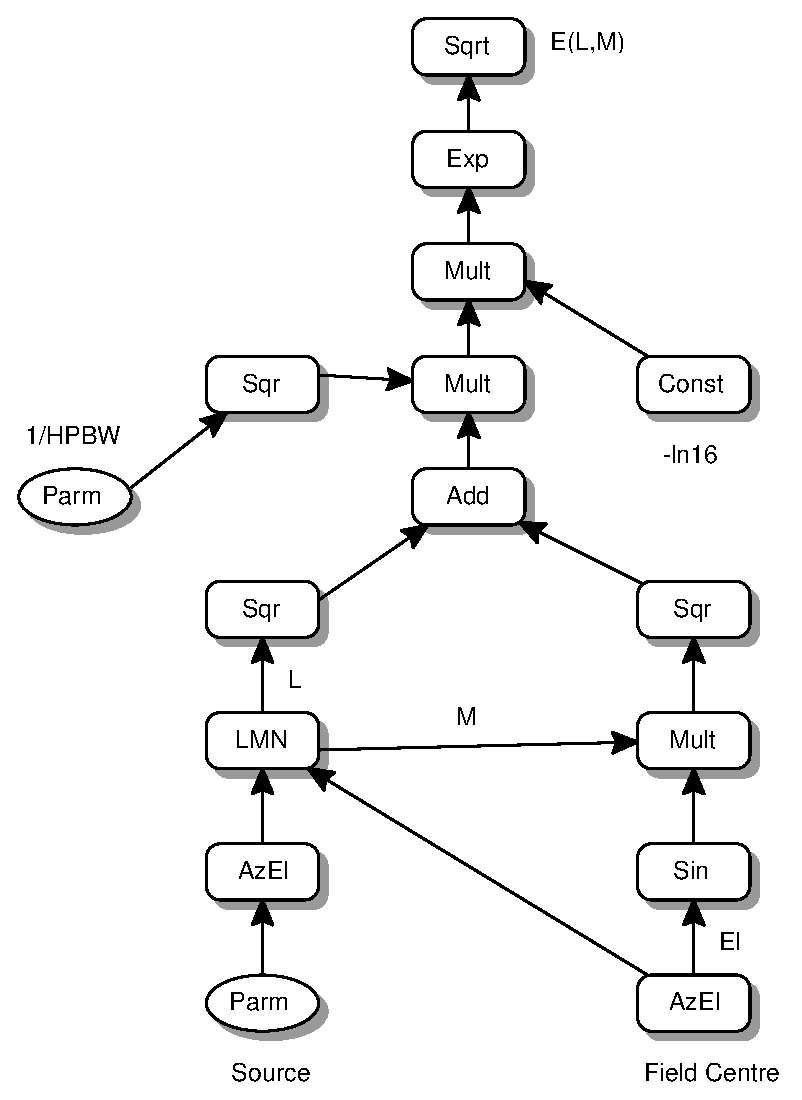
\includegraphics{LAR_MeqTree.eps}}
\par}
\end{slide}
%---------------------------------------------------------------------- SLIDE -

%---------------------------------------------------------------------- SLIDE -
\begin{slide}{Reduction Goals}
\begin{small}
\begin{itemize}
\item Left - most reduction packages; Right - MeqTrees
\end{itemize}
\end{small}
{\centering
\resizebox*{0.27\columnwidth}{!}{\includegraphics{3C449.ps}}
\resizebox*{0.27\columnwidth}{!}{\includegraphics{3C449_background.ps}}
\par}
\end{slide}
%---------------------------------------------------------------------------

%---------------------------------------------------------------------- SLIDE -
\begin{slide}{Know Thy E-Jones}
\begin{small}
\begin{itemize}
\item No longer acceptable to model primary beams as simple Gaussians
\item South Africa SKA Calibration and Imaging Workshop 2006 
\begin{itemize}
\item At least 4 or 5 presentations concerned with detailed measurements of telescope primary beams
\item Example - work of R. Reid et al. at DRAO on polarization leakage
\begin{itemize}
\item Each telescope of DRAO SST has different E-Jones voltage pattern
\item Detailed measurements made of the pattern for each dish
\item Accurate correction for instrumental polarization now possible   
\end{itemize}
\end{itemize}
\end{itemize}
\end {small}
\end{slide}
%------------------------------------------------------------------------------

%---------------------------------------------------------------------- SLIDE -
\begin{slide}{DRAO Stokes I}
{\centering
\resizebox*{0.6\columnwidth}{!}{\includegraphics{stokes_I.ps}}
\par}
\end{slide}
%------------------------------------------------------------------------------

%---------------------------------------------------------------------- SLIDE -
\begin{slide}{Stokes U No Correction}
{\centering
\resizebox*{0.6\columnwidth}{!}{\includegraphics{stokes_two.ps}}
\par}
\end{slide}
%------------------------------------------------------------------------------

%---------------------------------------------------------------------- SLIDE -
\begin{slide}{Stokes U Corrected}
{\centering
\resizebox*{0.6\columnwidth}{!}{\includegraphics{stokes_one.ps}}
\par}
\end{slide}
%------------------------------------------------------------------------------

%---------------------------------------------------------------------- SLIDE -
\begin{slide}{Know Thy FPA E-Jones}
\begin{small}
\begin{itemize}
\item Detailed knowledge of individual FPA voltage patterns allows
accurate `first order' prediction of phased array beam shapes
\begin{itemize}
\item Resampling and interpolation tools allow extrapolation from 
coarse `grid' measurements of actual FPA elements to finer grid for 
prediction of actual values associated with radio sources in the field
\end{itemize}
\item Assuming MIRANdA / SKA dishes and receiver elements are stamped out of 
uniform molds, detailed measurements of FPA voltage patterns on 
`representative' dishes should allow us to model entire array.
\item GRASP calculations are the equivalent of the above activity for
purposes of the simulations presented here.
\end{itemize}
\end {small}
\end{slide}
%------------------------------------------------------------------------------


%---------------------------------------------------------------------- SLIDE -
\begin{slide}{Simulated FPA}
\begin{small}
\begin{itemize}
\item 30 dipole elements in each of X and Y directions
\item Frequency = 1500 MHz; Spacing = lambda / 2
\item Dish diameter = 10m; Focal length = 4.5m
\item No coupling between elements; No feed struts in simulation
\item Not meant as a `realistic' final FPA design, but a good
testbed for various aspects of software development and data processing
\end{itemize}
\end {small}
{\centering
\resizebox*{0.4\columnwidth}{!}{\includegraphics{dipole_array_layout.ps}}
\par}
\end{slide}
%------------------------------------------------------------------------------

%---------------------------------------------------------------------- SLIDE -
\begin{slide}{Simulation Procedure}
\begin{small}
\begin{itemize}
\item Do GRASP calculations of voltage radiation patterns for each of the 
X and Y dipoles used in this simulation
\begin {itemize}
\item We get both co-polarization and cross-polarization leakage terms
\end{itemize}
\item Convert GRASP `grd' files to FITS images
\item MeqTrees reads in radiation patterns from the FITS images
\item Phase up X and Y radiation patterns, depending on optimization criteria,
for requested observing position. In most of the simulations shown here 
we observe on a 5 x 5 grid centred on L=M=0, in steps of 82 arcmin (HPBW). 
\item Form E-Jones Matrix (fully complex) from weighted combinations
\item Simulate observations of the `visible' sky via our equation:
\end{itemize}
\begin{displaymath}
  \vvCoh\ssIJ 
  ~= 
  ~\mjBeam\ssI
  ~\vvIQUV
  ~\mjBeam\ssJ^\ast
\end{displaymath}
\end {small}
\end{slide}
%------------------------------------------------------------------------------

%---------------------------------------------------------------------- SLIDE -
\begin{slide}{Typical GRASP Dipole Pattern}
\begin{small}
\begin{itemize}
\item In reality, we must measure these patterns in order to do accurate 
predicts, and thus compare with observations
\end{itemize}
\end {small}
{\centering
\resizebox*{0.65\columnwidth}{!}{\includegraphics{Voltage_pat1.ps}}
\par}
\end{slide}
%------------------------------------------------------------------------------

%---------------------------------------------------------------------- SLIDE -
\begin{slide}{Sky Coverage}
\begin{small}
\begin{itemize}
\item Basically we can attempt to do beam-forming over the range -0.05 to 0.05 radians in L and M.
\end{itemize}
\end {small}
{\centering
\resizebox*{0.6\columnwidth}{!}{\includegraphics{sky_coverage_linear.ps}}
\par}
\end{slide}                             
%---------------------------------------------------------------------- SLIDE -

%---------------------------------------------------------------------- SLIDE -
\begin{slide}{Phase Conjugate Weighting - I}
\begin{small}
\begin{itemize}
\item Phase conjugate weighting maximizes gain in observed
direction, but does nothing particular for beam shape
\item demo shows I beams for central row as we move from left edge toward centre of array in steps of 82 arcmin (HPBW)
\end{itemize}
\end {small}
{\centering
\resizebox*{0.3\columnwidth}{!}{\includegraphics{I_11.ps}}
\resizebox*{0.3\columnwidth}{!}{\includegraphics{I_12.ps}}
\resizebox*{0.3\columnwidth}{!}{\includegraphics{I_13.ps}}
\par}
\end{slide}

%---------------------------------------------------------------------- SLIDE -

%---------------------------------------------------------------------- SLIDE -
\begin{slide}{Phase Conjugate Weighting - I}
\begin{small}
\begin{itemize}
\item Phase conjugate weighting maximizes gain in observed
direction, but does nothing particular for beam shape
\item demo shows I beams for middle row as we move from left edge toward centre of array in steps of 82 arcmin (HPBW)
\end{itemize}
\end {small}
{\centering
\resizebox*{0.3\columnwidth}{!}{\includegraphics{I_16.ps}}
\resizebox*{0.3\columnwidth}{!}{\includegraphics{I_17.ps}}
\resizebox*{0.3\columnwidth}{!}{\includegraphics{I_18.ps}}
\par}
\end{slide}

%---------------------------------------------------------------------- SLIDE -

%---------------------------------------------------------------------- SLIDE -
\begin{slide}{Phase Conjugate Weighting - I}
\begin{small}
\begin{itemize}
\item Phase conjugate weighting maximizes gain in observed
direction, but does nothing particular for beam shape
\item demo shows I beams as we move along top edge of array in steps of 82 arcmin (HPBW)
\end{itemize}
\end {small}
{\centering
\resizebox*{0.3\columnwidth}{!}{\includegraphics{I_21.ps}}
\resizebox*{0.3\columnwidth}{!}{\includegraphics{I_22.ps}}
\resizebox*{0.3\columnwidth}{!}{\includegraphics{I_23.ps}}
\par}
\end{slide}
%---------------------------------------------------------------------- SLIDE -

%---------------------------------------------------------------------- SLIDE -
\begin{slide}{Phase Conjugate Weighting - Q}
\begin{small}
\begin{itemize}
\item demo shows Q response for central row as we move from left edge toward centre of array in steps of 82 arcmin (HPBW)
\end{itemize}
\end {small}
{\centering
\resizebox*{0.3\columnwidth}{!}{\includegraphics{Q_11.ps}}
\resizebox*{0.3\columnwidth}{!}{\includegraphics{Q_12.ps}}
\resizebox*{0.3\columnwidth}{!}{\includegraphics{Q_13.ps}}
\par}
\end{slide}

%---------------------------------------------------------------------- SLIDE -

%---------------------------------------------------------------------- SLIDE -
\begin{slide}{Phase Conjugate Weighting - Q}
\begin{small}
\begin{itemize}
\item demo shows Q response for middle row as we move from left edge toward centre of array in steps of 82 arcmin (HPBW)
\end{itemize}
\end {small}
{\centering
\resizebox*{0.3\columnwidth}{!}{\includegraphics{Q_16.ps}}
\resizebox*{0.3\columnwidth}{!}{\includegraphics{Q_17.ps}}
\resizebox*{0.3\columnwidth}{!}{\includegraphics{Q_18.ps}}
\par}
\end{slide}

%---------------------------------------------------------------------- SLIDE -

%---------------------------------------------------------------------- SLIDE -
\begin{slide}{Phase Conjugate Weighting - Q}
\begin{small}
\begin{itemize}
\item demo shows Q response as we move along top edge of array in steps of 82 arcmin (HPBW)
\end{itemize}
\end {small}
{\centering
\resizebox*{0.3\columnwidth}{!}{\includegraphics{Q_21.ps}}
\resizebox*{0.3\columnwidth}{!}{\includegraphics{Q_22.ps}}
\resizebox*{0.3\columnwidth}{!}{\includegraphics{Q_23.ps}}
\par}
\end{slide}
%---------------------------------------------------------------------- SLIDE -

%---------------------------------------------------------------------- SLIDE -
\begin{slide}{Optimized Gaussian Beam - I}
\begin{small}
\begin{itemize}
\item Obtain values for phase-conjugate weighting in a particular direction
\item Provide these values as initial guess for weights to MeqTrees solver
\item Solver adjusts weights until phased beam has optimal gaussian shape
\item demo shows I beams for central row as we move from left edge toward centre of array in steps of 82 arcmin (HPBW)
\end{itemize}
\end {small}
{\centering
\resizebox*{0.3\columnwidth}{!}{\includegraphics{I_gauss_11.ps}}
\resizebox*{0.3\columnwidth}{!}{\includegraphics{I_gauss_12.ps}}
\resizebox*{0.3\columnwidth}{!}{\includegraphics{I_gauss_13.ps}}
\par}
\end{slide}

%---------------------------------------------------------------------- SLIDE -

%---------------------------------------------------------------------- SLIDE -
\begin{slide}{Optimized Gaussian Beam - I}
\begin{small}
\begin{itemize}
\item Obtain values for phase-conjugate weighting in a particular direction
\item Provide these values as initial guess for weights to MeqTrees solver
\item Solver adjusts weights until phased beam has optimal gaussian shape
\item demo shows I beams for middle row as we move from left edge toward centre of array in steps of 82 arcmin (HPBW)
\end{itemize}
\end {small}
{\centering
\resizebox*{0.3\columnwidth}{!}{\includegraphics{I_gauss_16.ps}}
\resizebox*{0.3\columnwidth}{!}{\includegraphics{I_gauss_17.ps}}
\resizebox*{0.3\columnwidth}{!}{\includegraphics{I_gauss_18.ps}}
\par}
\end{slide}

%---------------------------------------------------------------------- SLIDE -
%---------------------------------------------------------------------- SLIDE -
\begin{slide}{Optimized Gaussian Beam - I}
\begin{small}
\begin{itemize}
\item Obtain values for phase-conjugate weighting in a particular direction
\item Provide these values as initial guess for weights to MeqTrees solver
\item Solver adjusts weights until phased beam has optimal gaussian shape
\item demo shows I beams as we move along top edge of array in steps of 82 arcmin (HPBW)
\end{itemize}
\end {small}
{\centering
\resizebox*{0.3\columnwidth}{!}{\includegraphics{I_gauss_21.ps}}
\resizebox*{0.3\columnwidth}{!}{\includegraphics{I_gauss_22.ps}}
\resizebox*{0.3\columnwidth}{!}{\includegraphics{I_gauss_23.ps}}
\par}
\end{slide}

%---------------------------------------------------------------------- SLIDE -

%---------------------------------------------------------------------- SLIDE -
\begin{slide} {AzEl Telescope Simulation - I}
\begin{small}
\begin{itemize}
\item Calculate Parallactic Angle as a function of time for AzEl-mounted
telescope stationed at VLA site which tracks position RA = 0 hr, Dec = 0 deg
\item Phase up FPA at a position whose offset with respect to the
tracking centre is -0.02 radians in both L and M when the Parallactic Angle is zero (transit)
\item Adjust FPA phase conjugate weights to keep beam centred on this
position.
\begin{itemize}
\item 8 hour observation; calculate FPA beam every 10 minutes
\end{itemize}
\item Total Intensity beam shown for start, middle and end of observation 
\end{itemize}
\end {small}
{\centering
\resizebox*{0.3\columnwidth}{!}{\includegraphics{I_azel_1.ps}}
\resizebox*{0.3\columnwidth}{!}{\includegraphics{I_azel_24.ps}}
\resizebox*{0.3\columnwidth}{!}{\includegraphics{I_azel_48.ps}}
\par}
\end{slide}

%---------------------------------------------------------------------- SLIDE -

%---------------------------------------------------------------------- SLIDE -
\begin{slide} {AzEl Telescope Simulation - Q}
\begin{small}
\begin{itemize}
\item Calculate Parallactic Angle as a function of time for AzEl-mounted
telescope stationed at VLA site which tracks position RA = 0 hr, Dec = 0 deg
\item Phase up FPA at a position whose offset with respect to the
tracking centre is -0.02 radians in both L and M when the Parallactic Angle is zero (transit)
\item Adjust FPA phase conjugate weights to keep beam centred on this
position.
\begin{itemize}
\item 8 hour observation; calculate FPA beam every 10 minutes
\end{itemize}
\item Q response shown for start, middle and end of observation 
\end{itemize}
\end {small}
{\centering
\resizebox*{0.3\columnwidth}{!}{\includegraphics{Q_azel_1.ps}}
\resizebox*{0.3\columnwidth}{!}{\includegraphics{Q_azel_24.ps}}
\resizebox*{0.3\columnwidth}{!}{\includegraphics{Q_azel_48.ps}}
\par}
\end{slide}

%---------------------------------------------------------------------- SLIDE -

%---------------------------------------------------------------------- SLIDE -
\begin{slide}{Modcal - Remove Anything}
\begin{itemize}
\item Algorithm developed at DRAO to get rid of unwanted sources when you don't have a good understanding of your E-Jones.
\item Baseline-based rather than antenna-based so not really part of the Jones Matrix formalism.
\item Can be useful as a method of last resort.
\item Only about 20 lines of python code with MeqTrees.
\end{itemize}
\end{slide}
%------------------------------------------------------------------------------

%---------------------------------------------------------------------- SLIDE -
\begin{slide}{Modcal - Example}
\begin{small}
\begin{itemize}
\item Right image shows source in sidelobe which does not clean properly; left image shows source vaporised by modcal algorithm.
\end{itemize}
\end {small}
{\centering
\resizebox*{0.9\columnwidth}{!}{\includegraphics{modcal_demo.ps}}
\par}
\end{slide}
%------------------------------------------------------------------------------


%---------------------------------------------------------------------- SLIDE -
\begin{slide}{Conclusion: Know Thy E-Jones}
\begin{itemize}
\item Heuristics
\item Learning
\end{itemize}
\end{slide}
%------------------------------------------------------------------------------
%---------------------------------------------------------------------- SLIDE -
\begin{slide}{What's Next?}
\ptsize{10}
\begin{itemize}
\item Need Better Optimization than Gaussian Beam
\begin{itemize}
\item Spheroids
\item Kaiser-Bessel
\end{itemize}
\item Generate GRASP models of antennas more suitable for FPA such
as Vivaldis and simulate observations with them.
\item Look at effects of system gain variations on formed beams.
\end{itemize}
`Solving for the Hubble constant (say as a polc in time) should be
possible too, but you need a machine big enough to model the universe
on....'

- Oleg M Smirnov, Russian/Dutch computer scientist
\end{slide}
%---------------------------------------------------------------------- SLIDE -

%---------------------------------------------------------------------- SLIDE -
\begin{slide}{Questions?}
\begin{itemize}
\item Email: tony.willis@nrc.ca
\end{itemize}
\end{slide}                             
%---------------------------------------------------------------------- SLIDE -

%---------------------------------------------------------------------- SLIDE -
\begin{slide}{Acknowledgements}

\begin{small}
\begin{itemize}
\item MeqTrees team, especially Oleg Smirnov, Maaijke Mevius and Sarod Yatawatta for assistance on MeqProblems related to focal plane arrays
\item Jan Noordam for aips++ Note 185 on the Measurement Equation
\item Bruce Veidt for GRASP calculations and advice on antenna-related issues
\item 3C449 image made (a long time ago) at the VLA, operated by NRAO / AUI / NSF
\end{itemize}
\end{small}
\end{slide}
%---------------------------------------------------------------------- SLIDE -
\end{document}


\end{document}

